\documentclass[a4paper,10pt]{article}


\usepackage{t1enc}
\usepackage{linguex}
\usepackage{harvard}
\usepackage{graphicx}
\usepackage{amsmath}
\usepackage{amssymb}
\usepackage{graphicx}
\usepackage{tikz}
\usepackage{subfigure}
\usepackage{eurosym}






%opening
\title{Exp1}
\author{Fabian Schlotterbeck}

\begin{document}

\maketitle



\section{Introduction}
The present experiment was a picture verification experiment. It served two purposes. Firstly, we wanted to see whether the findings of \citeasnoun{Chemlatoappear} could be replicated using a different method. In particular, we collected truth value judgments about set diagrams instead of acceptability ratings and also included distractor items in order to keep participants from developing strategies. Secondly, we tested another type of linguistic construction which has not yet been investigated experimentally. These were constructions  like \Next containing {\it every} embeded under the non-monotone operator {\it exactly one}. The scalar item {\it every} is the utmost item in its scale. There has been a debate about whether constructions like these should give rise to global scalar implicatures like in \NNext \citeaffixed{}{see}.

\ex. \a.[]   Exactly one student was parsised by all the teachers. 

\ex. \a.[$\rightsquigarrow$] It is not true that exactly one student was praised by some teachers. 

\subsection{Procedure}
The present experiment was part of a dual task experiment employing picture verification and a sternberg task \cite{Sternberg1966}. In addition to the picture verification task participants had to solve a memory task in some trials. In the {\it high load} condition participants had to remember six letters while performing the picture verification. In the {\it low load} condition they had to remember one letter and in the {\it no load} condition they didn't have to remember anything while they were performing the picture verification. In the {\it memory only} conditions they only had to perform a memory task (ie. remember one or six letters) but no picture verification. All the critical items of the present experiment were presented in the {\it no load} condition. Only distractor items were presented in one of the dual task conditions.  

In each trial participants were first asked to indicate readiness by pressing a button. In the {\it no load} condition, after they had pressed the button an  asterisk was flashed on the screen six times within $7.2s$. Then a sentence and a picture were presented simultaneously. Within $12s$ participants had to judge whether the sentence was true with respect to the picture. They indicated their judgment by pressing one of two buttons. After they had provided their judgment the next trial started automatically. If they did not respond within twelve seconds, the next trial was started. Judgments and reaction times were logged.

In the {\it low load} and {\it high load} condition a trial looked similar to a trial in the {\it no load} condition except for two things. Firstly, in the dual task conditions instead of asterisks letters were flashed on the screen. Secondly, after finishing the picture verification task a question appeared on the screen probing for a letter. Participants had to indicate by pressing a button whether they thought the letter had been present in the array from the beginning of the trial.

Except for one thing, the {\it memory only} trials were identical to the dual task trials. In {\it memory only} trials the picture verification part was replaced with a blank screen. That is, in the middle of such trials the screen stayed blank for $5s$. 

The experiment started with a practise session consisting of $25$ trials devided into three blocks (1st block: memory task only, ten trials; 2nd block: picture verification only, five trials; 3rd block: dual task, ten trials). Then one list consisting of 249 trials devided into three blocks was presented. An experimental session took about 75 minutes. During the whole experiment no feedback was provided to the participants.

\subsection{Materials}

There were three sentence conditions. An example of each sentence condition is given in \ref{ex:AE}$-$\ref{ex:EA}. We will refer to the sentence type in \ref{ex:AE} as the $\forall \exists$ type of sentence. Such sentences contained the determiner {\it einige} (some) embedded under {\it jeder} (every). Sentences like the one in \ref{ex:EE}  contained {\it einige} embedded under {\it genau ein} (exactly one), they will be referred to as $\exists ! \exists$ sentences. Finally, sentences like in \ref{ex:EA}  containig {\it jeder} embedded under {\it genau ein} will be referred to as $\exists ! \forall$.  Within every one sentence the two quantificational determiners were separated by a clause boundary as to enforce linear scope readings. We constructed 48 experimental items, so  48 sentences of each type were constructed yielding a total of 144 sentences.

Because of the logical relations between the different readings of the sentences in \ref{ex:AE}$-$\ref{ex:EA}, it was not possible to construct all types of disambiguating diagrams one might wish to test. However, testing some of the possible sentence-picture combinations can already provide crucial information about the status of global and local implicatures of embedded scalar items. Below we will introduce the picture materials for each sentence condition in turn. Every sentence was paired with diagrams of four types. In total, this yielded twelve conditions and 576 pictures. The conditions were distributed over twelve lists accordding to a latin square design ensuring that in each list every item was only present in one condition. In addition to the target sentences, 201 (?) distractors were included in each list. Of these, $n$ were {\it memory only} trials. One third (?) of them was presented in the {\it no load} condition, another third (?) in the {\it low load} and $n$ in the {\it high load} condition. The picture verification of {\it n} of the distractor items was intended to yield a "yes true" response, $n$ were false.
\small
\exg. \label{ex:AE}F{\"u}r jeden dieser Umweltsch{\"u}tzer gilt: er  boykottierte einige dieser Gro{\ss}konzerne.\\
For each of\ these environmentalists holds: he boycotted some of\ these conglomerates.\\
 Each of\ these environmentalists boycotted some of\ these conglomerates.\\

\exg. \label{ex:EE}F{\"u}r genau einen dieser Umweltsch{\"u}tzer gilt: er bykottierte einige dieser Gro{\ss}konzerne.\\
For exactly one of\ these environmentalists holds: he boycotted some of\ these conglomerates.\\
 Exactly one of\ these environmentalists boycotted some of\ these conglomerates.\\

\exg. \label{ex:EA}F{\"u}r genau einen dieser Umweltsch{\"u}tzer gilt: er bykottierte jeden dieser Gro{\ss}konzerne.\\
For exactly one of\ these environmentalists holds: he boycotted each of\ these conglomerates.\\
Exactly one of\ these environmentalists boycotted eachl of\ these conglomerates.\\

\normalsize

\subsubsection{Diagrams for $\forall \exists$ sentences}

The $\forall \exists$ sentences were paired with diagrams like those in Figure \ref{fig:AE}. Figure \ref{fig:AE-LITGLBLOC} is compatible with the global implicature, the local implicature and the literal meaning of \ref{ex:AE}. Using the terminology of \citename{Chemlatoappear} we will refer to such diagrams as {\it strong} diagrams. In contrast to {\it strong} diagrams, Figure \ref{fig:AE-LITGLB} is not compatible with the local implicature ({\it weak} diagrams) and Figure \ref{fig:AE-LIT} is only compatible with the literal meaning of the sentence ({\it literal} diagrams). Finally, Figure \ref{fig:AE-false} is not compatible with the sentence at all ({\it false} diagrams).  These four conditions constitute a replication of \citeasnoun[Experiment 1]{Chemlatoappear}.

\begin{figure}[ht]
\centering
\subfigure[{\it strong}: compatible with global, local and literal interpretation]{
\includegraphics[width=3.8cm]{./pictures/Umweltschuetzer01.eps}
\label{fig:AE-LITGLBLOC}
}
\subfigure[{\it weak}: compatible with global, literal but not with local interpretation]{
\includegraphics[width=3.8cm]{./pictures/Umweltschuetzer02.eps}
\label{fig:AE-LITGLB}
}
\subfigure[{\it literal}: Only compatible with the literal meaning]{
\includegraphics[width=3.8cm]{./pictures/Umweltschuetzer03.eps}
\label{fig:AE-LIT}
}
\subfigure[{\it false}: Not compatible with the sentence at all]{
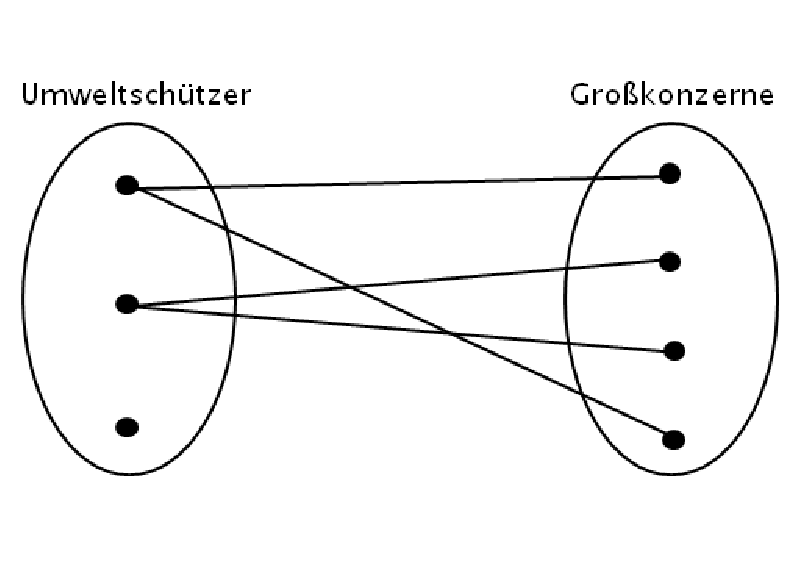
\includegraphics[width=3.8cm]{./pictures/Umweltschuetzer04.eps}
\label{fig:AE-false}
}
\caption[Optional caption for list of figures]{Diagrams for $\forall \exists$ sentences}
\label{fig:AE}
\end{figure}

\subsubsection{Diagrams for $\exists! \exists$ sentences}

The $\exists! \exists$ sentences were paired with digrams like those in Figure \ref{fig:EE}. The diagram in Figure \ref{fig:EE-LITGLBLOC} is compatible with all three interpretations.  We use \possessivecite{Chemlatoappear} term {\it all} to refer to such diagrams. Figure\ref{fig:EE-LOC} is only compatible with the local interpretation ({\it local} diagrams) and Figure \ref{fig:EE-LIT} is only compatible with the literal interpretation ({\it literal} diagrams). Figure \ref{fig:EE-false} is plainly false with respect to the sentence in \ref{ex:EE} ({\it false} diagrams). These four conditions replicate  \citeasnoun[Experiment 2]{Chemlatoappear}.

\begin{figure}[ht]
\centering
\subfigure[{\it all}: compatible with global, local and literal interpretation]{
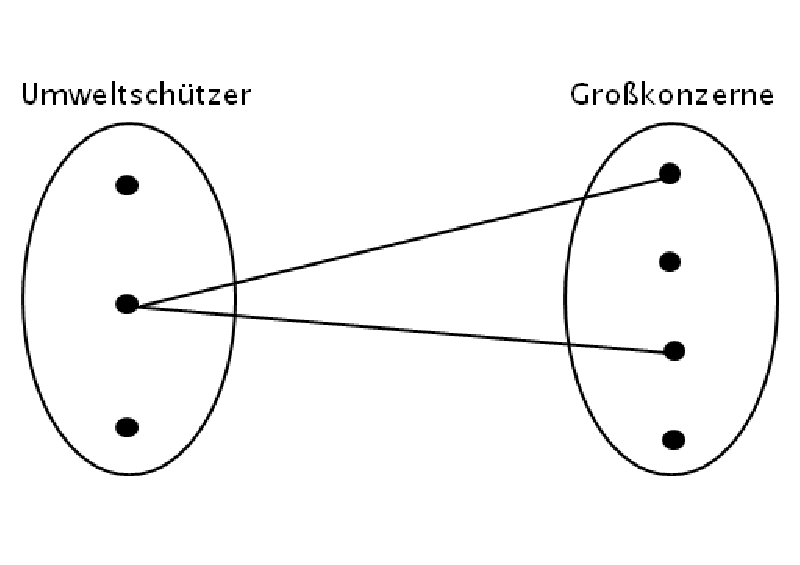
\includegraphics[width=4cm]{./pictures/Umweltschuetzer05.eps}
\label{fig:EE-LITGLBLOC}
}
\subfigure[{\it local}: compatible with local interpretation only]{
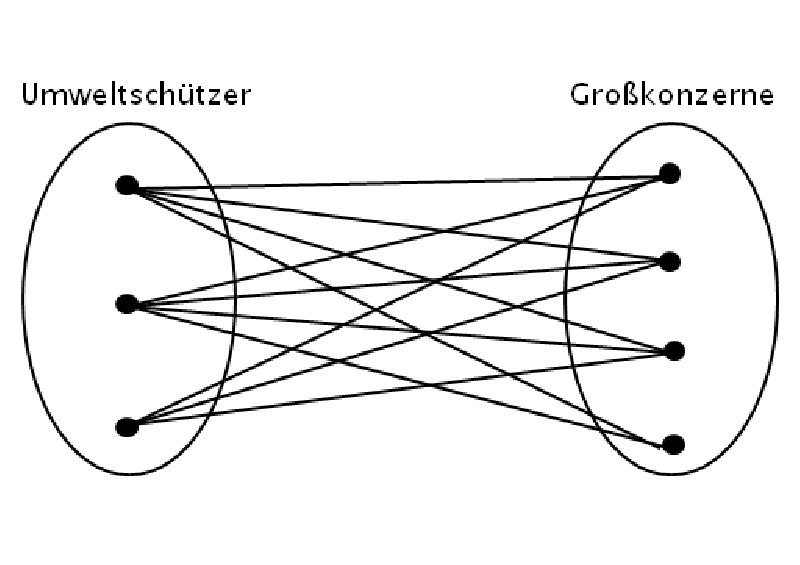
\includegraphics[width=4cm]{./pictures/Umweltschuetzer06.eps}
\label{fig:EE-LOC}
}
\subfigure[{\it literal}: compatible with literal interpretation only]{
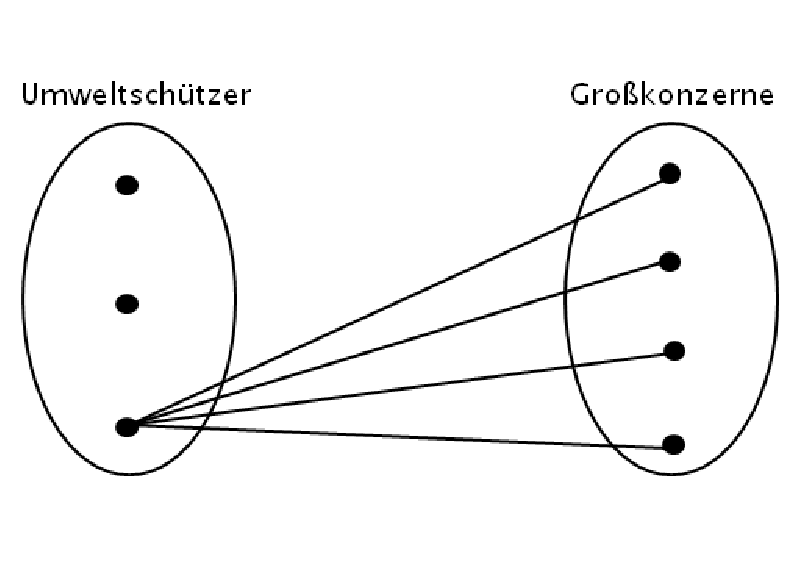
\includegraphics[width=4cm]{./pictures/Umweltschuetzer07.eps}
\label{fig:EE-LIT}
}
\subfigure[{\it all}: not compatible at all]{
\includegraphics[width=4cm]{./pictures/Umweltschuetzer08.eps}
\label{fig:EE-false}
}
\caption[Optional caption for list of figures]{Diagrams for $\exists! \exists$ sentences}
\label{fig:EE}
\end{figure}

\subsubsection{Diagrams for $\exists! \forall$ sentences}

The $\exists! \forall$ sentences were paired with digrams like those in Figure \ref{fig:EA}. Figure \ref{fig:EA-LIT} is only true under the literal reading ({\it literal} diagrams) while  Figure \ref{fig:EA-LITGLB} is only true with respect to the global implicature ({\it global} diagrams), denying the weaker scalar alternative containig {\it einige} (some). Diagrams like those in Figures \ref{fig:EA-FALSE1} and \ref{fig:EA-FALSE2} were not compatible with the $\exists! \forall$ sentences. Figure \ref{fig:EA-FALSE1} is incompatible because there are too few connections. Figure \ref{fig:EA-FALSE2} is incompatible because there are too many connections. We used two types of incompatible pictures only because of thechnical reasons.

\begin{figure}[ht]
\centering
\subfigure[compatible with literal meaning and global implicature]{
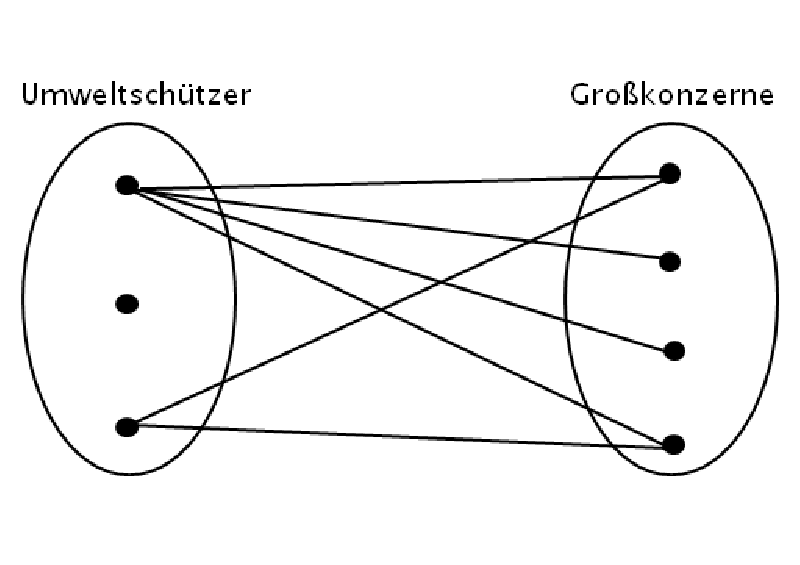
\includegraphics[width=4cm]{./pictures/Umweltschuetzer09.eps}
\label{fig:EA-LIT}
}
\subfigure[compatible with literal interpretation only]{
\includegraphics[width=4cm]{./pictures/Umweltschuetzer10.eps}
\label{fig:EA-LITGLB}
}
\subfigure[false because of insufficient connections]{
\includegraphics[width=4cm]{./pictures/Umweltschuetzer11.eps}
\label{fig:EA-FALSE1}
}
\subfigure[false because of to many connections]{
\includegraphics[width=4cm]{./pictures/Umweltschuetzer12.eps}
\label{fig:EA-FALSE2}
}
\caption[Optional caption for list of figures]{Diagrams for $\exists! \forall$ sentences}
\label{fig:EA}
\end{figure}

\subsection{Participants}
60 native German speakers (40 female, mean age: $24$, ranging between $20$ and $40$) from the University of T{\"u}bingen participated in the study. Participants were na\"ive to the purpose of the study. They were paid \euro{10} compensation. 

\subsection{Hypotheses and Predictions}
Since most of the present experiment replicates the study of \citeasnoun{Chemlatoappear}, the major hypotheses and predictions can be found therein. We will shortly summarize the main points here. In monotone increasing environments local implicatures do generally imply global implicatures, but not reversely.  In these cases the distinction between local and global accounts is rather subtle. It is hard to test the existence of locally drawn implicatures in upward entailing contexts empirically \citeaffixed{Chemlatoappear,Geurts2009}{see, however,}. The same applies to the existence of global implicatures in upward entailing contexts. Generally, if one reading implies another one and both are rated equally, nothing can be concluded since the sentences may just be ambiguous.

If we do find evidence for the existence of global scalar implicatures, this does at least provide evidence that strict locality is not enough. This is because when applied to sentences containing embedded scalar items, local accounts are not able to generate global implicatures. If implicature computation was strictly local, global implicatures should not be drawn. 

The heterogenity of global accounts is another complicating factor.  Global accounts differ with respect to the readings they assume to be possible in upward entailing environments. Some global accounts \citeaffixed{}{eg.} posit global strategies that produce readings equivalent to eg. the local implicature of $\forall \exists$ sentences. Other more restricted global accounts do not manage to generate any of the local readings. Therefore, it is not possible to decide between globality and locality by testing scalar items in upward entailing contexts. Even clear evidence for so called local readings does only discard some global accounts, but not globality in general. 

In non-monotone contexts implication from local to global readings does not hold. Furthermore, no global account can generate any of the local readings in such contexts. Therefore, as \citename{Chemlatoappear} point out, non-monotone contexts are a good test case. If local implicatures are detected in such environments, strict globality is clearly insufficient. 

Yet another distinction within the global accounts can be drawn on the basis of sentences like \ref{ex:EA} which have not been investigated experimentally thus far. Replacing {\it jeder} (every) in \ref{ex:EA} with any other item from its scale does not yield a sentence that entails the original one. Therefore, most theories do not consider this substitution an alternative to be negated by implicature. Some global accounts do, however, allow for such implicatures. Luckily, for sentences like \ref{ex:EA}  global readings do not imply literal readings. Therefore acceptance of global readings of such sentences would have straightforward theorectical implications. We will now spell out the predictions for each sentence condition in some detail.

\subsubsection{Predictions for $\exists! \forall$ sentences}
Local accounts let us predict that {\it strong} diagrams are accepted more often than {\it literal} ones.  Furthermore, they do not predict any difference between acceptance of {\it literal} and {\it weak} diagrams. Global accounts, on the other hand, predict that {\it  weak} diagrams are accepted more often than {\it literal} diagrams. At least more restricted global accounts do not predict any difference between {\it strong} and {\it weak} diagrams.

\subsubsection{Predictions for $\exists! \forall$ sentences}
Global accounts predict that {\it all} diagrams are rated better than {\it literal} diagrams. They cannot explain more acceptance of {\it local} diagrams than of {\it false} diagrams. Local accounts predict both {\it all} and {\it local} diagrams to be rated better than {\it litaral} and false {\it diagrams}.


\subsubsection{Predictions for $\exists! \forall$ sentences}
Some global accounts would predict {\it global} pictures to be rated better than {\it literal} pictures. Other global accounts do not predict any difference. Since the literal reading is true in both types of diagrams, they should be rated better than {\it false1} and {\it false2}.


\subsection{Results}

Overall participants were able to solve the task. In the distractor items the picture verification was done accurately in $88\%$ ($sd: 33\%$) of the cases. All participants were above $70\%$ and significantly better than chance. On average it took participants $4989ms$ ($sd:2176ms$) to come up with their answer in the filler trials. We will now consider results for the three sentence conditions in turn.

\subsubsection{Results for $\exists! \forall$ sentences}
The judgment pattern we obtained for $\exists! \forall$ sentences is depicted in Figure \ref{fig:EABars}. The {\it strong} diagrams were judged to be true in $90\%$ of the cases, {\it weak} diagrams received "yes" judgments in $79\%$ , {\it literal} diagrams in  $72\%$  and {\it false} in $0.9\%$.  A logit mixed effects model with binomial link function containing a fixed effect of {\it diagram} as well as random effects of items and participants revealed a clear effect of {\it diagram}. In particular {\it false}, {\it literal} and {\it weak} diagrams all received fewer "yes" judgments than {\it strong} diargams (all $p<.001$).  Another logit mixed effects model only modelling data for {\it literal} and {\it weak} diagrams also revealed an reliable effect of {\it diagram} (p<.05). Finally, a model only considering  {\it false} and {\it literal} diagrams also revealed a significant effect of {\it diagram} (p<.001).

\begin{figure}[ht]
\centering
\subfigure[$\forall\exists$ sentences]{
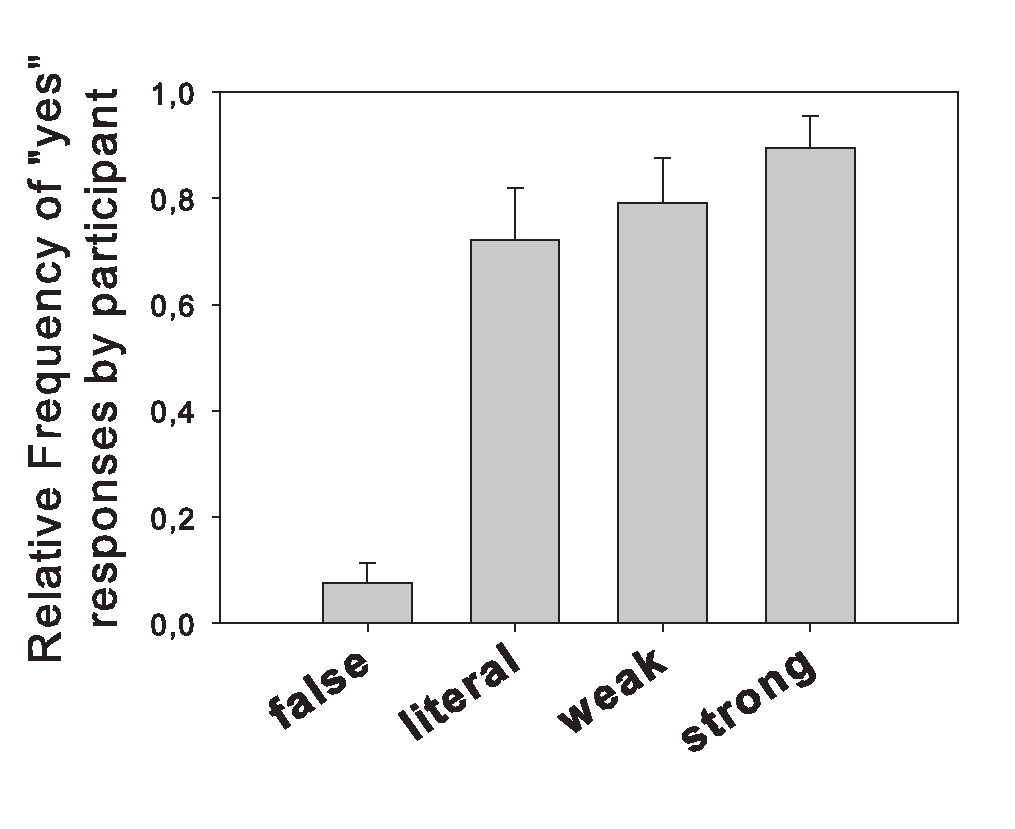
\includegraphics[width=3.92cm]{../data/JudgmentsAllSomeBars.eps}
\label{fig:EABars}
}
\subfigure[$\exists! \exists$ sentences]{
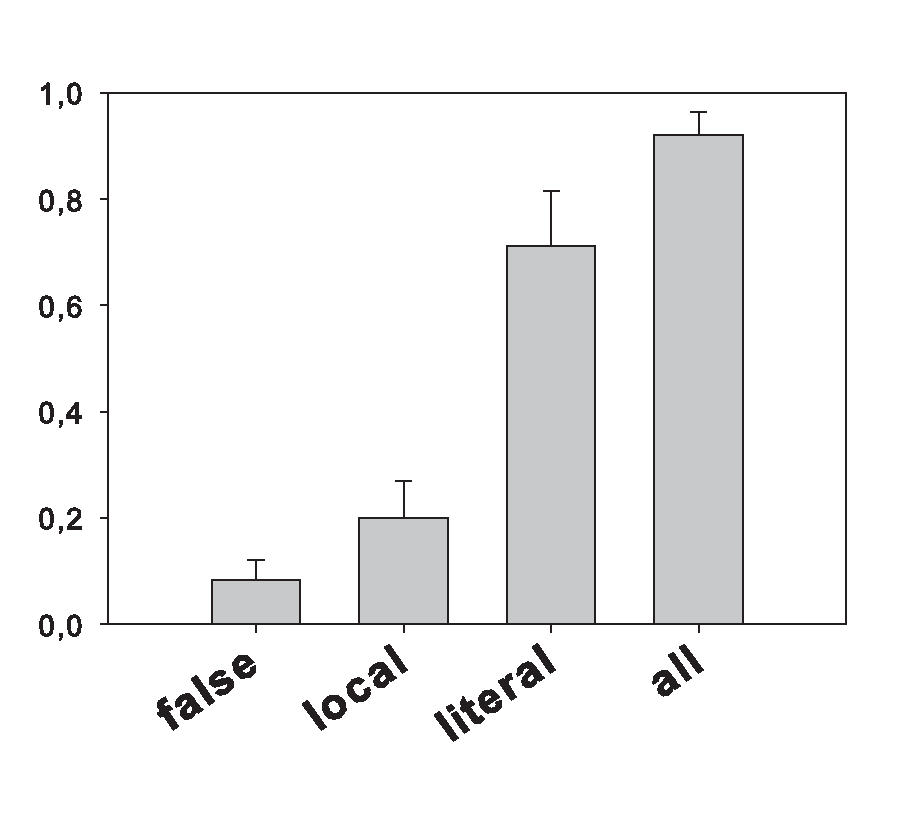
\includegraphics[width=3.5cm]{../data/JudgmentsExactlySomeBars.eps}
\label{fig:EEBars}
}
\caption[Optional caption for list of figures]{Mean judgments}
\label{fig:Bars}
\end{figure}

\subsubsection{Results for $\exists! \exists$ sentences}
The response pattern for $\exists! \exists$ sentences is presented in Figure \ref{fig:EEBars}. Unsurprisingly, these sentences were accepted as truthfull description of {\it false} diagrams in only $0.8\%$ of all cases. The {\it local} diagrams received  "yes" responses in $20\%$, {\it literal} in $71\%$ and {\it all} in $93\%$ of the time. A logit mixed effects model with {\it diagram} as fixed effect as well as item and participant as random effects revealed a signficant effect of {\it diagram}. The {\it all}, {\it literal} and {\it local} diagrams were all accepted more often than the {\it false} diagram (all $p<.001$). A simpler model only considering {\it local} and {\it literal} diagrams reveald a reliable effect of {\it diagram} (p<.001) as did a model only considering {\it literal} and {\it all} diagrams (p<.001).

\subsubsection{Tendency for acceptance of diagrams compatible with local readings}
Participants who accepted {\it local} diagrams together with $\exists! \exists$ sentences also on average made a greater difference between {\it strong} and {\it weak} diagrams when they were judging $\forall \exists$ sentences. This is reflected in a significant positive correlation between these two variables. The first variable is the proportion of "yes" responses per participant to the {\it local} diagrams in the $\exists! \exists$ sentences. The second one is the difference per participant between the proportion of "yes" responses to {\it strong} and {\it weak} diagrams in the $\exists! \exists$ sentences. This correlation ($p<.001$) is visualized in Figure \ref{fig:cor}. 

\begin{figure}[t]
\begin{center}
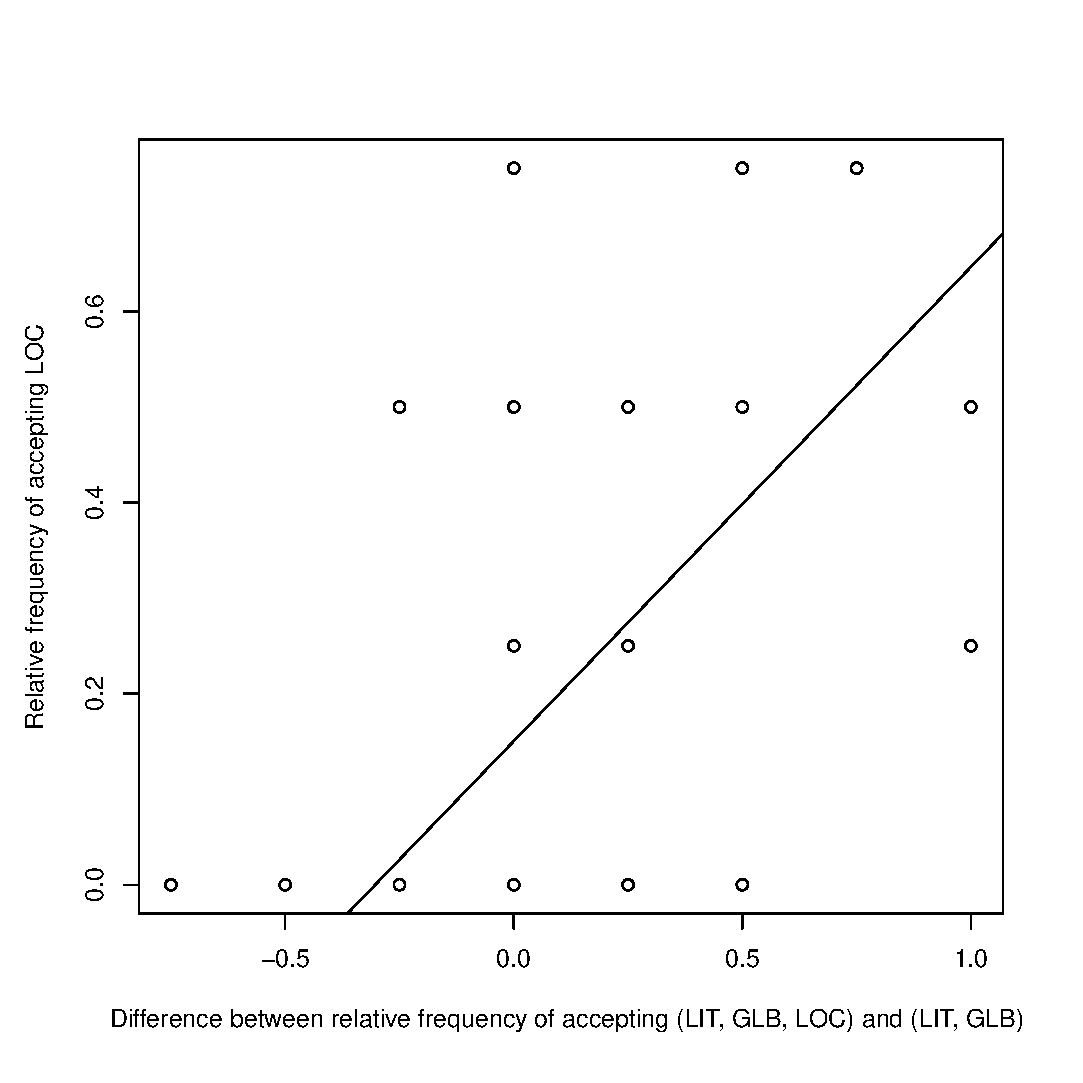
\includegraphics[width=3.92cm]{../data/KorrelationScatterPlot.eps}
\end{center}
\label{fig:cor}
\caption{Correlation}
\end{figure}

\bibliographystyle{harvard}
\bibliography{ESI}
\end{document}
